%!TEX root = ../document.tex
\chapter{Evaluation}\label{ch:evaluation}

\begin{quotation}
  {\small\it }"Always design a thing by considering it in its next larger context - a chair in a room, a room in a house, a house in an environment, an environment in a city plan."{\small\it -- Eliel Saarinen, Finnish Architect }
\end{quotation}

In this chapter, we go through our qualitative and quantitative evaluation of browserCloudjs system, comparing it to our initial goals and expectations.

\section{Qualitative assessment}

In a qualitative perspective, browserCloudjs performs successfully the following:

\begin{itemize}
    \item Efficient resource discovery through peer-2-peer routing over a structured overlay network, using a DHT.
    \item Distribute Jobs through the peers available, submiting, coordinating and aggregating the results.
    \item Remove the need for centralized indexes or points of control. There is still a need of a rendezvous point to enable new peer joins, however the data transmited, computed and stored inside the network is peers responsability.
    \item Enable every machine equiped with a WebRTC enabled browser to be part of a browserCloudjs instance. In 2013, the number of WebRTC capable devices already exceed one billion\footnote{Google I/O presentation in 2013 - https://bloggeek.me/webrtc-next-billion/}
    \item Enable peers to both participate and contribute to a job and at the same time submiting and requesting the network to process their own.
    \item Enable browsers to be part of one or more browserCloudjs instance.
    \item browserCloudjs' Job Scheduler is job agnostic, this means that different types of jobs can be executed on demand without any previous configuration or preparation.
    \item browserCloudjs solves the decentralized communication problem between browsers in a scalable way, giving the opportunity for new scenarios to be developed on top of it through its modular and pluggable approach.
\end{itemize}

We've developed a Demo video of browserCloudjs working, this video can be seen at https://www.youtube.com/watch?v=kjwIjoENCR .

\section{Quantitative assessment}

In this section we evaluate browserCloud.js via real executions on top of increasing number of browsers executing locally, to assess the limits of current Javascript engines on typical desktop machines, and with micro-benchmarks to determine the speedups that can be achieved in distributed executions with one browser per individual desktop machine.

\subsection{The setup}

In order to assess the potential of the proposed system, we have built a ray-tracing application, adapted from algorithms available, written in full vanilla JavaScript, that can be run on any typical modern browser engine. This algorithm allows us to stress-test the CPU,  and the possibility to obtain advantages through processing parallelism. We need this to understand whether the expected speeds up resulting from distributing the tasks through the browserCloud.js peers network, are not hindered by loosing efficiency due to message routing on the overlay Network.

The setup used during the tests was a system running Chrome version 39 on a Intel Processor Code i7 2.3Ghz with 16Gb of RAM. The STUN server used was provided by Google.

\subsection{Goals}

Following our motivation to build browserCloudjs in the first place, that is, to provide a way to take advantage of the volunteer computing paradigm, using the idle resources available on user machines, leveraging the capabilities that offered to us by the Web Platform, we set ouselves with some goals to proove if our solution is viable, through:

\begin{itemize}
    \item Measuring the time lapsed for a single browser to compute a CPU bound job and several browsers to compute that same job, but in parallel.
    \item Measuring the RTT time between any of two browsers in the network and evaluate as routing efficiency evolves with the increase in number of browser
    \item Assessing if there are significant speedups
\end{itemize}

\subsection{Results}

We've perfomed tests in order to assess:

\begin{itemize}
    \item Time elapsed during a distributed ray-tracing job, checking for how it changed when we increased the number of browsers and the level of granularity in which we divided the job. Seen in Figures~\ref{fig:ray25}~,~\ref{fig:ray2500}~,~\ref{fig:ray25time}~and~\ref{fig:ray2500time}.
    \item How much time each ray-tracing task takes. Seen in Figure~\ref{fig:avgtimeexec}.
    \item What is the average round trip time between any of two browsers in a 10 browser network. Observed in Figure~\ref{fig:rtt}.
\end{itemize}

\begin{figure}[h!]
  \centering
  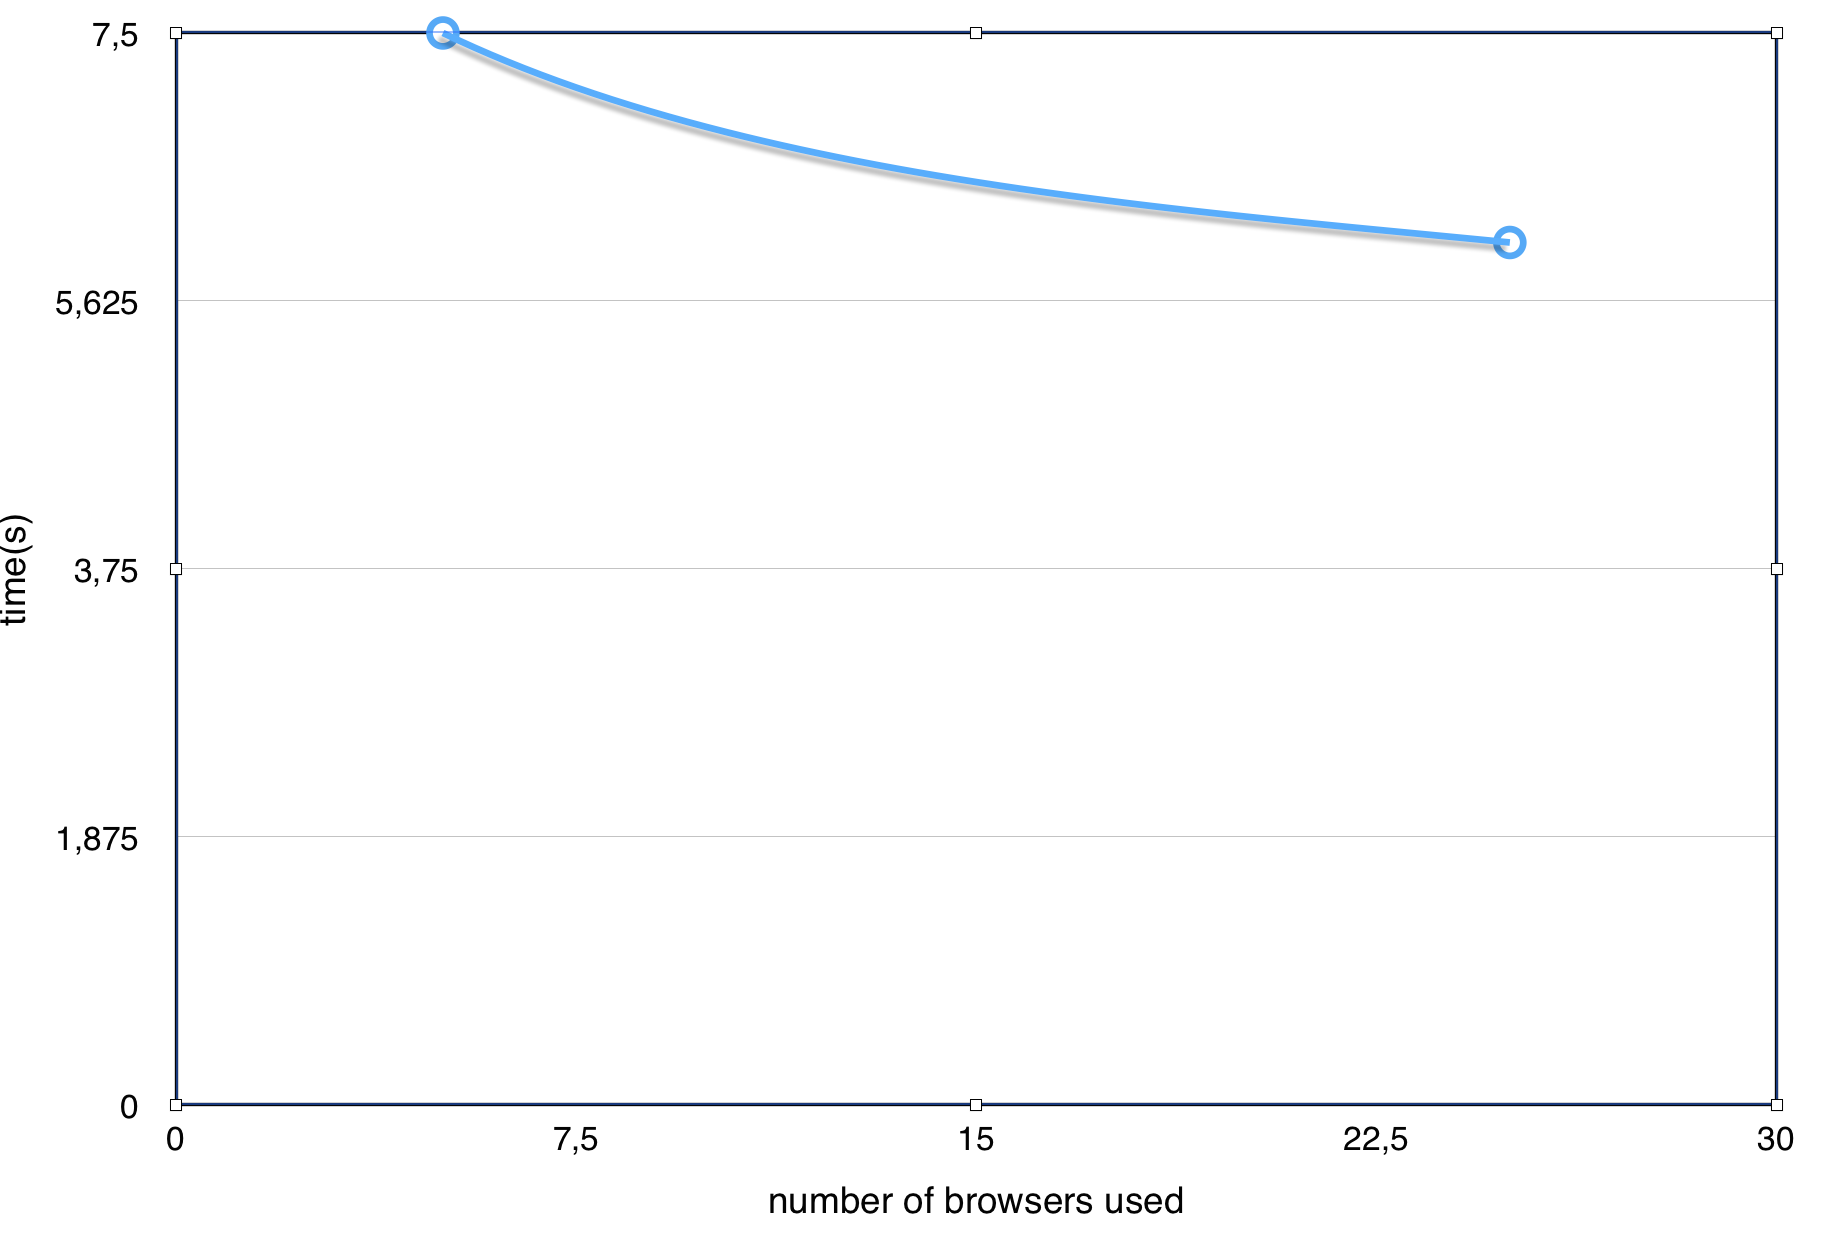
\includegraphics[width=0.8\textwidth]{figs/2.png}
  \caption{Time elapsed on a ray-tracing job divided in 25 computing units}
  \label{fig:ray25}
\end{figure}

\begin{figure}[h!]
  \centering
  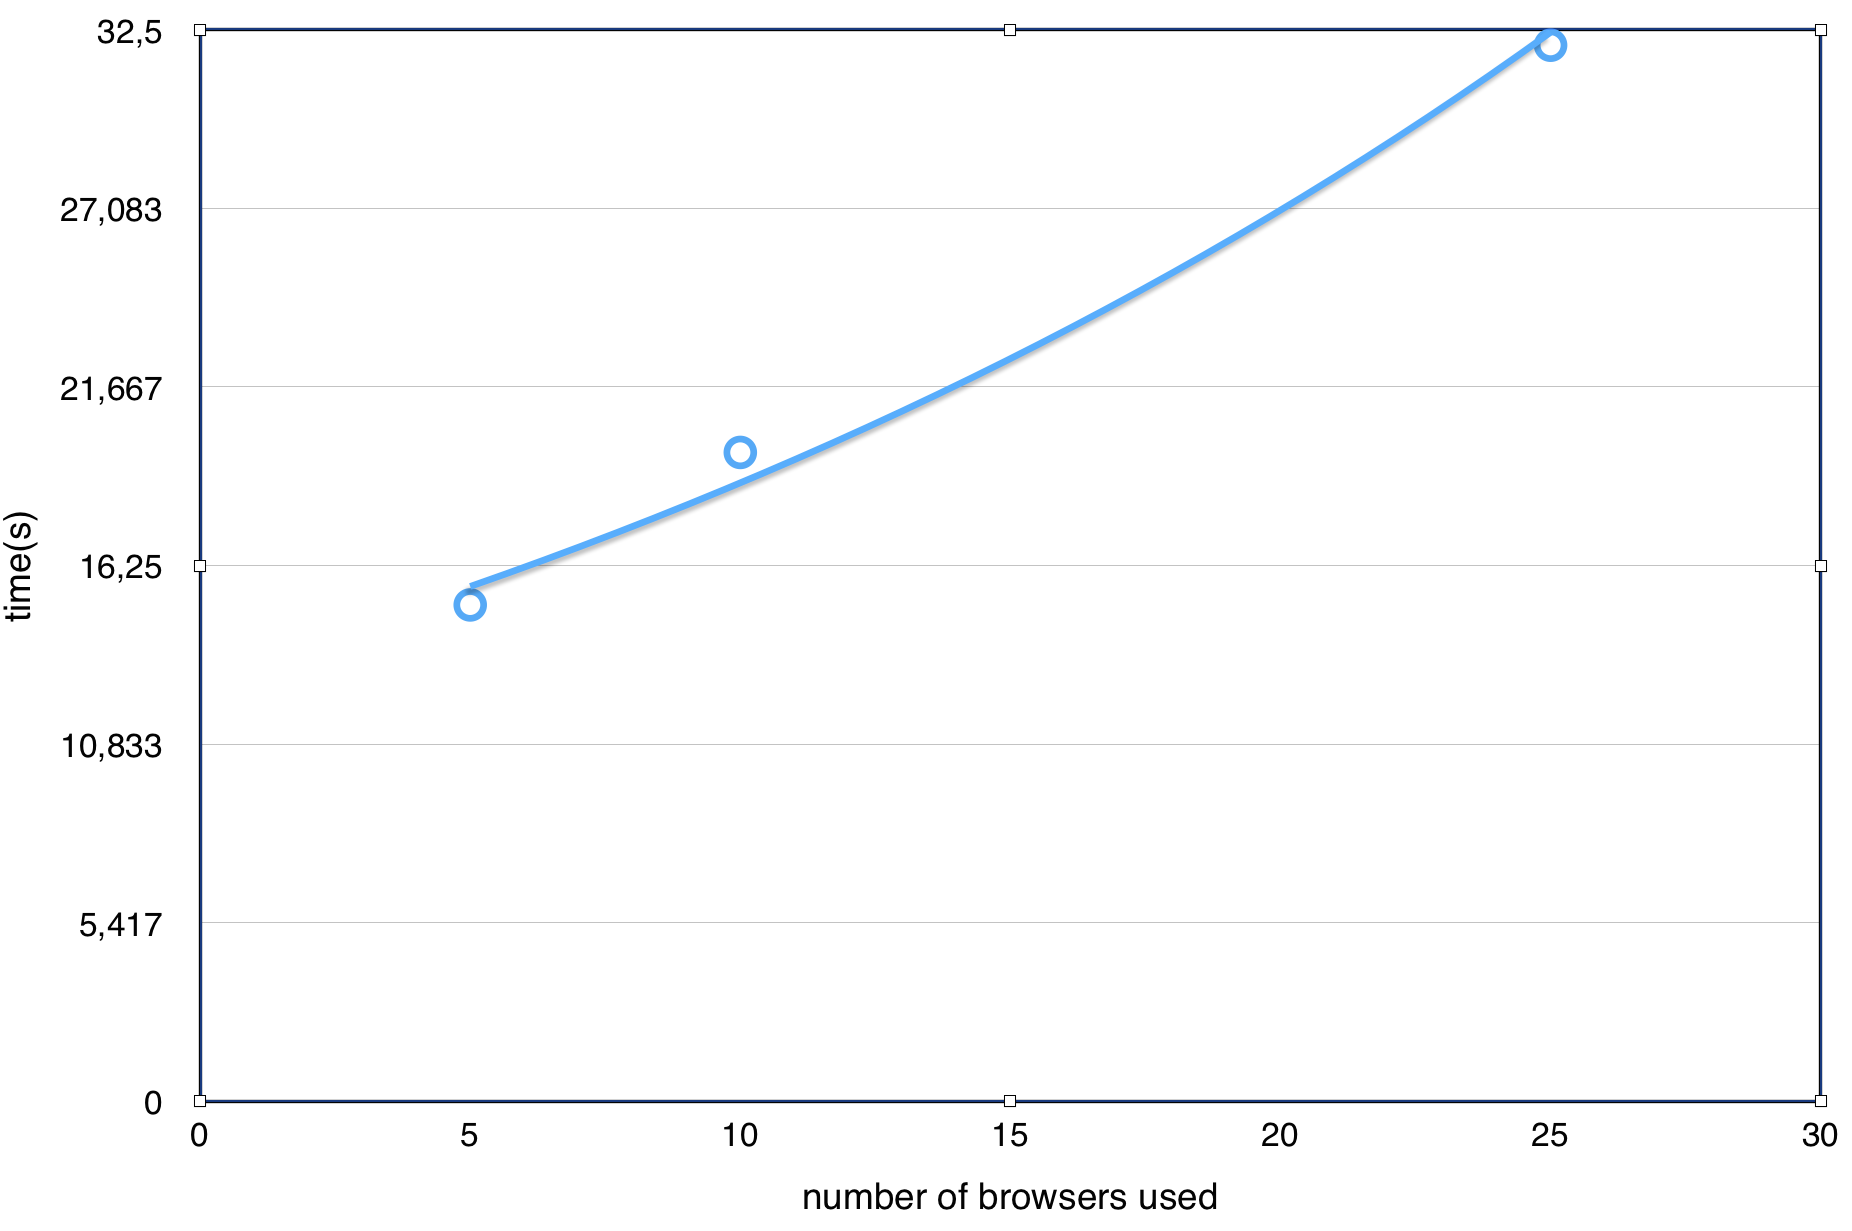
\includegraphics[width=0.8\textwidth]{figs/1.png}
  \caption{Time elapsed on a ray-tracing job divided in 2500 computing units}
  \label{fig:ray2500}
\end{figure}

\begin{figure}[h!]
  \centering
  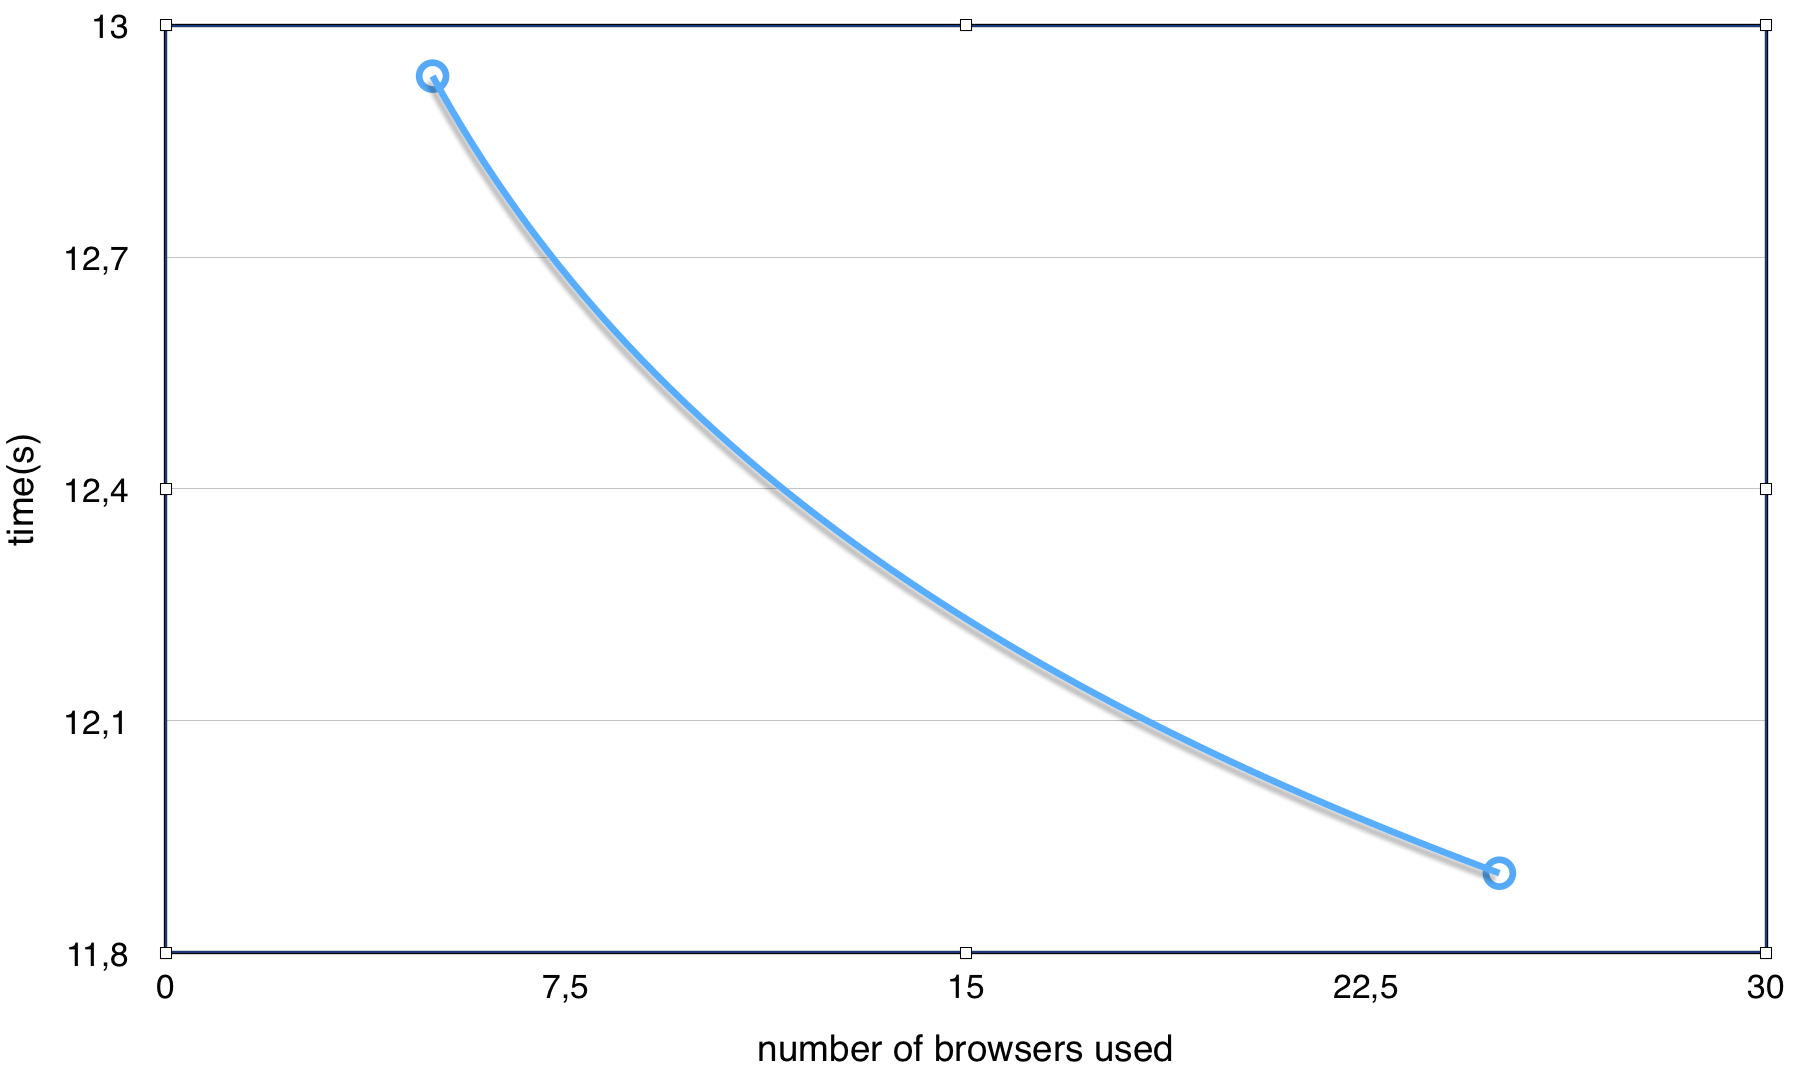
\includegraphics[width=0.8\textwidth]{figs/4.png}
  \caption{Time elapsed on a ray-tracing job divided in 25 computing units (with induced web RTT delay)}
  \label{fig:ray25time}
\end{figure}


\begin{figure}[h!]
  \centering
  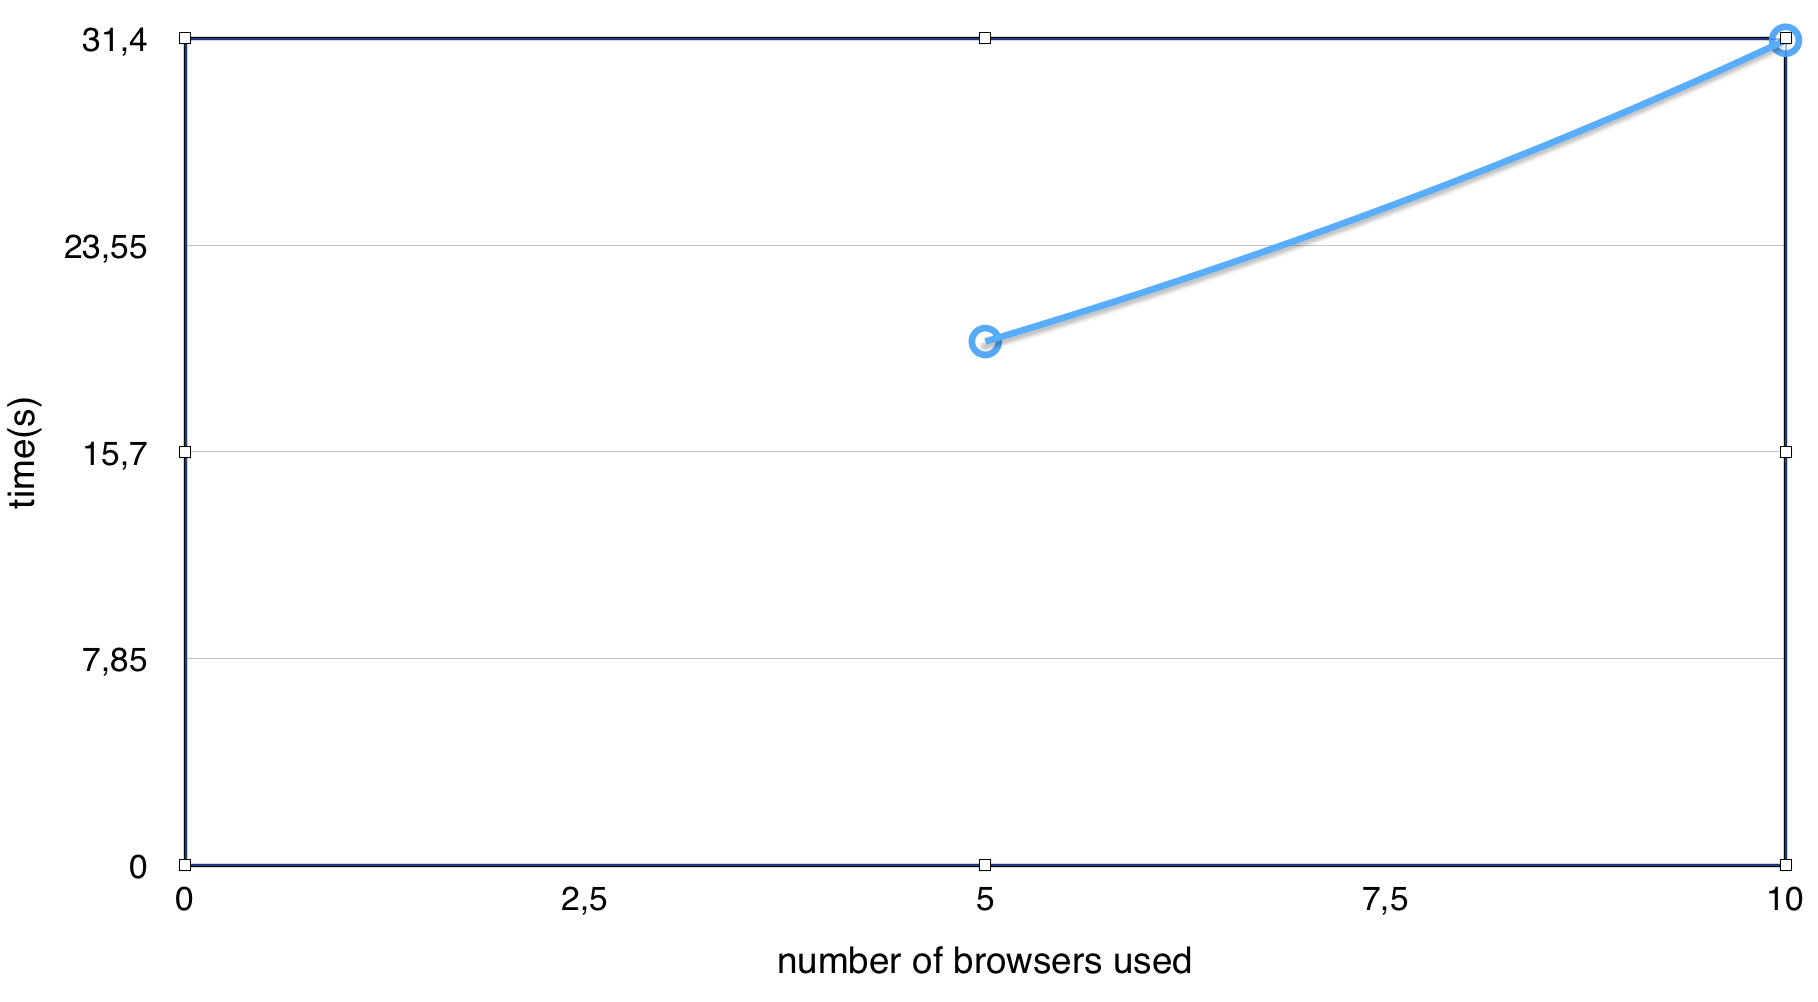
\includegraphics[width=0.8\textwidth]{figs/3.png}
  \caption{Time elapsed on a ray-tracing job divided in 2500 computing units (with induced web RTT delay)}
  \label{fig:ray2500time}
\end{figure}



\begin{figure}[h!]
  \centering
  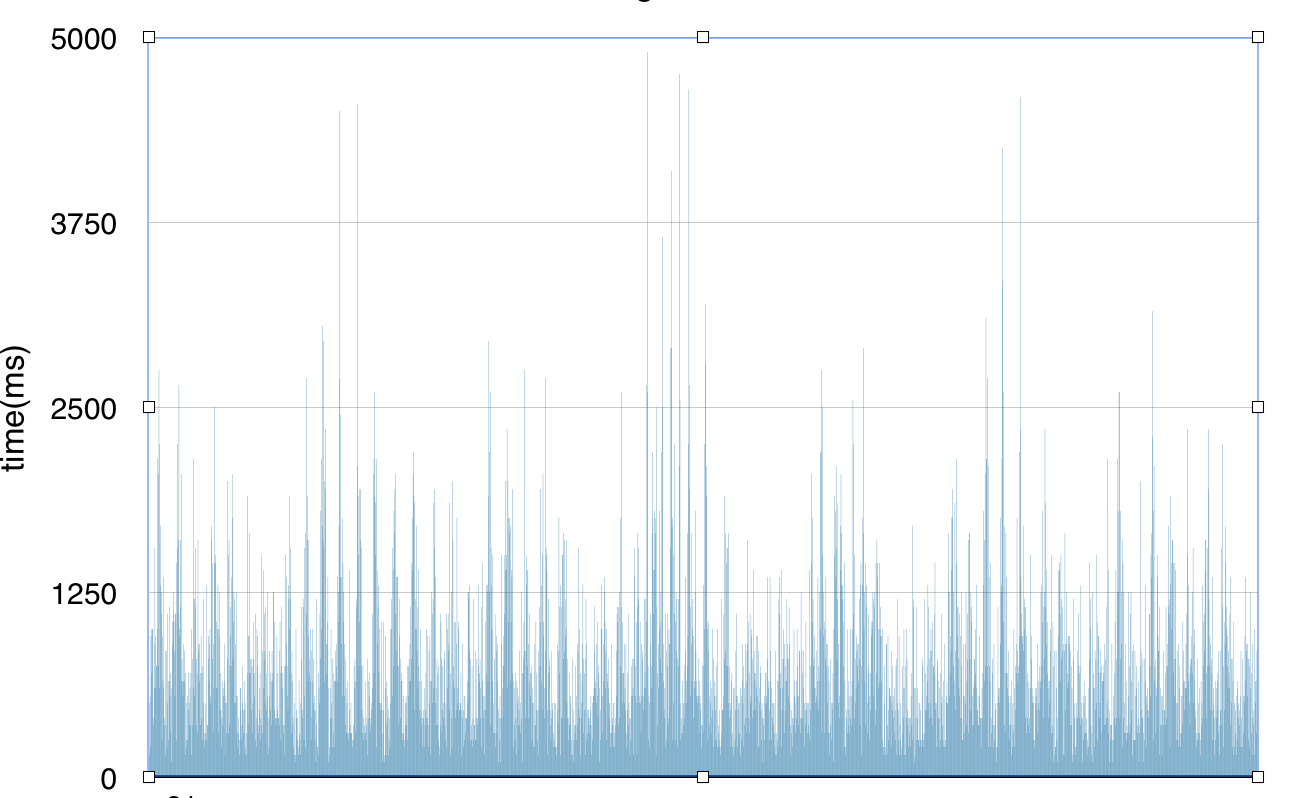
\includegraphics[width=0.8\textwidth]{figs/avg_time_exec.png}
  \caption{Average time for a task execution for a job fragmented in 2500 computing units}
  \label{fig:avgtimeexec}
\end{figure}

\begin{figure}[h!]
  \centering
  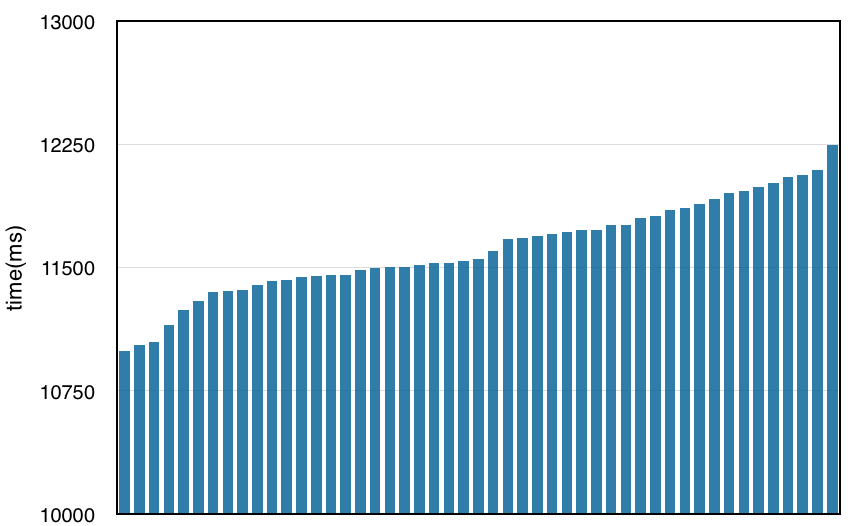
\includegraphics[width=0.8\textwidth]{figs/rtt.png}
  \caption{Average Round Trip Time between an two nodes in a 10 browser network}
  \label{fig:rtt}
\end{figure}

\subsection{Analysis}

The standard ray-tracing job using the algorithm developed, running in a single browser takes as median 23610.434ms to complete. As we can see in Figures~\ref{fig:ray2500}~and~\ref{fig:ray2500time}, our system excels in delivering faster results by dividing the job up to 2500 computational units (or tasks) and requesting from the browsers available in the network to compute those (i.e., a rectangle of the resulting output image). This is expected as ray-tracing is a known case of an embarrassingly parallel application.

One fact interesting to note is that we obtained much better results by reducing the granularity of which ray-tracing job was divided into, as we can see on Figures~\ref{fig:ray25}~and~\ref{fig:ray25time}. This happens due to two factors: a) the first is that since we have a lower number of tasks to be run by other browsers, we reduce the message routing overhead between nodes (i.e., resource discovery does not take so long); b) the second factor is that since this system was tested using a single machine and a networked simulated delay. When the number of tasks is too large, the workers in the browser are in fact competing for CPU resources (to execute tasks and to forward messages among them). This creates a scenario, where more nodes/workers actually  make the system slower, since this is a much more strict and resource constrained scenario, than a real example with browsers executing in different machines.

In a real world example, the actual execution time would be bounded by:\\

$\textbf{jobTime}=slowestDelayFromResourceDiscovery+timeOfExecutingSlowestTask+slowestDelayFromResultReply (1)$ \\

with full parallelism, where in our test scenario we have: \\

$\textbf{jobTime}=\sum{DelayFromResourceDiscovery}+(TimeOfExecuting\_N\_Tasks\_on\_M\_Resources)+\sum{DelayFromResultReply} (2)$\\

where N=2500 and M=8 hardware threads, therefore contention for CPU becomes higher with more nodes (browsers) as more messaging is taking place, besides the parallelized computation.

In a real world scenario, with more browsers from more machines, the total execution time (makespan) of a ray-tracing job would be closer to that described by Equation 1. It would be influenced by the maximum round trip time between any two nodes (so that the information for every task can be received and processed by another node), plus the time it would take to execute the most of CPU intensive task (e.g., the rectangle in the frame that has the more complex geometry and light reflections to be processed). Figures~\ref{fig:avgtimeexec}~and~\ref{fig:rtt} show what is the average task length and RTT between any two nodes, being the maximum for the first 61ms and the second 11174ms, creating a total of 11235ms (or 11.296s overall). This is a significant increase of efficiency, comparing to the sequential execution and also to the previous single-machine experiments.

It is important to note that in Figure~\ref{fig:avgtimeexec}, we can see several task execution lengths due to the complexity of each task, with more or less light reflections. With this microbenchmark we see that the execution time of each task, without any resource contention (1 node = 1 browser per machine), the task duration has an even lower upper bound (lower than 5s). This would entail the upper bound of total task execution time to be under 5061 ms (around just 5s), with a theoretical speedup of about 4.6 times (take into account that we would be using 2500 nodes then, so speedups are not perfectly linear due to communication overhead, as expected).

\subsection{Inference}

As we have discussed in the previous sections, we did managed to reach significant speedup between 2 and close to 5 times for our experiment, using only volunteer resources, that is a reduction between 50\% and 76\%.

When distributing a job through a multiple node network, one of the aspects we observed was that we can influence overall efficiency by adjusting how much resources we are going to take from the network to process the job, in this case, how much browsers. We also can influence it by deciding how much fine-grained each task it will be: the smaller the computation unit, the more we can distribute tasks through the network, with a natural trade-off of adding more task generation and messaging overhead, with diminishing returns when more and more, and smaller tasks are created. This has led us to understand and consider the opportunity for a premature job optimization tool, where a job would be particioned and distributed, depending on its size and complexity, with the goal of meeting the optimal point of the trade-off.

There are also some other performance bottlenecks we noticed that arise from the single threaded nature of JavaScript engines. These aspects are considered in our performance evaluation, such as:

\begin{itemize}
  \item Logging - Since V8 runs in a single thread, any synchronous operation will block the event loop and add delay to the whole processing, although these logs are essential for us to assess the efficiency of the infrastructure, they are not vital to the job.
  \item Delay added - One technique we used to simulate the network delay is to use the `setTimeout' native function of V8's JavaScript implementation, since this function is unable to receive floating millisecond values. Moreover, since `setTimeout' does not necessarily guarantee that the function will be executed in X amount of milliseconds, due to the nature of the event loop, there is always an extra delay added implicitly to the operation in the order of 1 to 3 ms.
  \item Tasks can not be sent in parallel - A node has to send each individual computing unit sequentially and independently, meaning that if we divide a job into 2000 for e.g, each task will have to wait for the previous to be sent.
  \item We've noticed a considerable machine resoures bottle neck when we had more than 40 data channels present in same machine - This means that is is unviable to levarage the full 48 fingers space our finger table has the capacity, since one fingers equals 2 data channels (one in and one out).
\end{itemize}

These bottlenecks were studied and will be tackled in future work, one of the solutions proposed is to use Service Workers\footnote{http://www.w3.org/TR/2014/WD-service-workers-20141118} for full multithreaded operation inside browserCloud.js.

\section{Finger Table Optimization for minimum number of hops between any two peers}

With our evaluation, we learned that a browser reaches a machine resource bottle neck when it comes to memory and CPU, when using more than 40 data channels simultaneously. As mentioned earlier, a finger in our Finger Table represents two data channels for a browser, one out and another in. This gives us the opportunity to study what can be the best approach in terms of finger selection from the options available, so we can optimize for the number of hops. We've picked 16 fingers (32 simultaneous data channels) as our limit per peer and studied the three following approaches:

\begin{itemize}
    \item A - Pick the first 16 fingers from a 48bit Finger Table
    \item B - Pick 16 fingers equality spaced in a 48bit Finger Table
    \item C - Pick 16 fingers using a geometric distribuion with decreasing density
\end{itemize}

For each of these approaches, we've evaluated the jump between a node and its fingers, the number of hops between a given peer and the peers between it and its fingers and finally, we measured the number minimum and the maximum of hops between any two peers.

\subsection{Pick the first 16 fingers from a 48bit Finger Table}

As we can observe in Table\ref{tab:table-a}, with this distribution with get a good minimum numer of hops between fingers of 1, but if a peer is beyond our finger table, we can reach a result of having to jump 33 additional hops in order to find that finger.

\begin{table}
    \centering
    \begin{tabular}{| c | c | c | c |}
    \hline
        Finger Level &  Finger Picked & Jump & Aditional hops for peers between fingers \\
        0 & 0 & 1 & 1 \\
        1 & 1 & 2 & 1 \\
        2 & 2 & 4 & 1 \\
        3 & 3 & 8 & 1 \\
        4 & 4 & 16 & 1 \\
        5 & 5 & 32 & 1 \\
        6 & 6 & 64 & 1 \\
        7 & 7 & 128 & 1 \\
        8 & 8 & 256 & 1 \\
        9 & 9 & 512 & 1 \\
        10 & 10 & 1024 & 1 \\
        11 & 11 & 2048 & 1 \\
        12 & 12 & 4096 & 1 \\
        13 & 13 & 8192 & 1 \\
        14 & 14 & 16384 & 1 \\
        15 & 15 & 32768 & 1 \\
        END & 48 & 281474976710656 & 33 \\
    \hline
    \end{tabular}
    \caption{Finger Table Distribution for first 16 fingers from a 48bit Finger Table}
    \label{tbl:table-a}
\end{table}

\subsection{Pick 16 fingers equality spaced in a 48bit Finger Table}

In this linear distribuition, seen in Table\ref{tab:table-b}, we have obtained a good stability when it comes to minimum and maximum of additional hops for peers between fingers, being constant of 3.

\begin{table}
    \centering
    \begin{tabular}{| c | c | c | c |}
    \hline
        Finger Level &  Finger Picked & Jump & Aditional hops for peers between fingers \\
        0 & 0 & 1 & 3 \\
        1 & 3 & 8 & 3 \\
        2 & 6 & 64 & 3 \\
        3 & 9 & 512 & 3 \\
        4 & 12 & 4096 & 3 \\
        5 & 15 & 32768 & 3 \\
        6 & 18 & 262144 & 3 \\
        7 & 21 & 2097152 & 3 \\
        8 & 24 & 16777216 & 3 \\
        9 & 27 & 134217728 & 3 \\
        10 & 30 & 1073741824 & 3 \\
        11 & 33 & 8589934592 & 3 \\
        12 & 36 & 68719476736 & 3 \\
        13 & 39 & 549755713888 & 3 \\
        14 & 42 & 4398046511104 & 3 \\
        15 & 45 & 35184372088832 & 3 \\
        END & 48 & 281474976710656 & 3 \\
    \hline
    \end{tabular}
    \caption{Finger Table Distribution for 16 fingers equality spaced in a 48bit Finger Table}
    \label{tbl:table-b}
\end{table}

\subsection{Pick 16 fingers using a geometric distribuion with decreasing density}

By using a non linear distribution, we have managed to decrease the optimal case for minimum additional hops necessary for peers between fingers, however, there was a tradeoff for fingers that are in the last section of our Finger Table, having an increased number of additional hops, comparing to the previous approach, as we can observe in Table~\ref{tab:table-c}.

\begin{table}
    \centering
    \begin{tabular}{| c | c | c | c |}
    \hline
        Finger Level &  Finger Picked & Jump & Aditional hops for peers between fingers \\
        0 & 0 & 1 & 1 \\
        1 & 1 & 2 & 1 \\
        2 & 2 & 4 & 1 \\
        3 & 3 & 8 & 1 \\
        4 & 4 & 16 & 2 \\
        5 & 6 & 64 & 2 \\
        6 & 8 & 256 & 2 \\
        7 & 10 & 1024 & 2 \\
        8 & 12 & 4096 & 4 \\
        9 & 16 & 65536 & 4 \\
        10 & 20 & 1048576 & 4 \\
        11 & 24 & 16777216 & 4 \\
        12 & 28 & 268435456 & 4 \\
        13 & 33 & 8589934592 & 5 \\
        14 & 38 & 274877906944 & 5 \\
        15 & 43 & 8796093022208 & 5 \\
        END & 48 & 281474976710656 & 5 \\
    \hline
    \end{tabular}
    \caption{Finger Table Distribution for 16 fingers using a geometric distribuion with decreasing density}
    \label{tbl:table-c}
\end{table}

\subsection{Inference}

From these 3 approaches, the second and the third approach have more interesting results, however, in order to pick the best for browserCloudjs, we have also to consider the number of total peers and what kind of messages are being used. For e.g, for a browserCloudjs instance focused on distributed computing, the second approach can be more interesting due to the natural implicit way of the network to load balance itself, due to the hashing function properties, however for a browserCloudjs instance focused on message routing or object storage/lookups, if a replication strategy such as DynamoDB or PAST is used, that is, replicating the objects to the following peers, having the knowledge of the consequent peers might be advantageous due to reduced number of hops for replica updates.

\section{Summary}

In this Chapter, we've discussed and presented our results when it comes to fullfilling the requirements we had initially to browserCloudjs. Starting with a qualitiative assessmentment, where we evaluate how browserCloudjs behaves and what functionalities does it offer, passing to a quantitative assessment, verifying that indeed there are speedups achieved by using browserCloudjs.
